\documentclass{llncs}
\usepackage{makeidx}
\usepackage{enumerate}
\usepackage[dvips,dvipdfm]{graphicx}
\usepackage{subfigure}
\usepackage{authblk}
\usepackage{amssymb}
\usepackage{amsmath}
\usepackage{amsfonts}
\usepackage{booktabs}
\usepackage{threeparttable}
\usepackage{algorithm}
\usepackage{algorithmicx}
\usepackage{algpseudocode}
\usepackage{textcomp}
\renewcommand{\algorithmicrequire}{\textbf{Input}}
\renewcommand{\algorithmicensure}{\textbf{Output}}
% \usepackage{fancyhdr}
% \pagestyle{fancy}
% \fancyhf{}
% \renewcommand{\headrulewidth}{0pt}
% \renewcommand{\footrulewidth}{0pt}
% \fancyhead[RO]{{\scriptsize Extended Refined Ordering Relations with Uncertainty \qquad\thepage}}
% \fancyhead[LE]{{\scriptsize \thepage\qquad Shuhao Wang, Lijie Wen, Zixuan Wang, Jianmin Wang and Jianwen Su}}
\begin{document}
\frontmatter 
\pagestyle{headings}
\addtocmark{Extended Refined Ordering Relations with Uncertainty}

\mainmatter
\title{A Behavioral Similarity Measure for Process Models based on Extended Refined Ordering Relations with Uncertainty}
\titlerunning{Extended Refined Ordering Relations with Uncertainty}

\author[$\$$]{Shuhao Wang}
\author[$\$$]{Lijie Wen}
\author[$\$$]{Zixuan Wang}
\author[$\$$]{Jianmin Wang}
\author[$\#$]{Jianwen Su}
\authorrunning{Shuhao Wang et al.}
\tocauthor{Shuhao Wang, Lijie Wen, Zixuan Wang, Jianmin Wang and Jianwen Su}
\affil[$\$$]{School of Software, Tsinghua University, Beijing 100084, P.R. China \authorcr
\texttt{shudiwsh2009@gmail.com,wenlj@tsinghua.edu.cn,
iamwangzixuan@hotmail.com,jimwang@tsinghua.edu.cn}}
\affil[$\#$]{Department of Computer Science, UC Santa Barbara, USA \authorcr
\texttt{su@cs.ucsb.edu}}
\institute{}

\maketitle

\begin{abstract}
Tao Jin has proposed new ordering relations between execution of tasks in business process models. He also gave an algorithm to compute the refined ordering relations for acyclic process models based on unfolding technology. However, his algorithm cannot work well for cyclic WF-nets and process models with invisible tasks. We extend his work and present a refinement of the relations. To better measure the differentiation between process models, we introduce the notion of sequential direct adjacency. Also, we propose an algorithm to compute relations in arbitrary WF-nets and utilize them to measure the similarity between process models.
\keywords{Business Process Model, Refined Ordering Relations with Uncertainty, Sequential Direct Adjacency, Behavioral Similarity}
\end{abstract}

\section{Introduction}\label{sec:introduction}

In a seminal paper \cite{jin2014computing}, Tao Jin has proposed new ordering relations between execution of tasks in business process models. He refines the causal and concurrency relations between two events in a concurrent system with uncertainty according to whether one task is always executed with the other task in the same instance. He then proposes some rules for adjacent tasks and some transitive laws for nonadjacent tasks, based on which he proposes an algorithm to compute the refined ordering relations for acyclic process models. The algorithm is done on the unfolding of a WF-net \cite{mcmillan1995technique,esparza1996improvement}.

Although Tao Jin' work is elegant, it has some drawbacks. First of all, for cyclic Petri nets, his algorithm cannot work well. According to his paper, the problem arises from the Global Fairness Assumption \cite{kindler1999liveness}. Secondly, invisible tasks have not been taken into consideration so that two models with different behavioral semantics may have the same set of ordering relations. To solve these problems, we extend his ordering relations to more trivial cases which is inspired by the work of DecSerFlow \cite{van2006decserflow}, and introduce the concept of sequential direct adjacency to better differentiate the behavioral semantics of two process models. Of course, we propose an algorithm to compute our relations in arbitrary WF-nets.

Furthermore, since our refined relations have a strong ability to represent the behavioral semantics of a process model and can efficiently measure the tiny differentiation between two models, even when they contain invisible tasks, we utilize them as a proper metric to measure the similarity between two process models.

Similarity measure can be widely used in many scenarios, such as model retrieval, process mining and model classification. There have been various proposals to this topic: based on textual information, the structure of process models, and their execution semantics \cite{kunze2011behavioral}.
% TODO: mainstream algorithms

In this paper, we propose a behavioral similarity measure based on the extended refined ordering relations with uncertainty. It satisfies metric properties, especially the triangle inequality \cite{zezula2006similarity}. The algorithm firstly extracts three types of relations and generates the relation sets of a process model. By measuring the similarity between relation sets of process models, a similarity value is finally given by the algorithm. We conduct experiments using process models from real enterprises and the results show that our similarity measure is both efficient and effective.

The remainder of this paper is structured as follows: 
% TODO: remainder of this paper

\section{Preliminaries}\label{sec:preliminaries}
Our work is to measure the similarity between two process models. There are many different notations to describe the business process, such as Business Process Model and Notation (BPMN), Event-driven Process Chain (EPC), Yet Another Workflow Language (YAWL) and Petri Net Markup Language (PNML). Since Petri net is suitable to analyze the behavior of process models, we will show our algorithm on Petri net. The concept of the Petri net has its origin in Carl Adam Petri's dissertation \cite{petri1966kommunikation}.

\begin{definition}[Petri net]\label{def:petrinet}
A Petri net is a triple $(P,T,F)$:
	\begin{itemize}
		\item[-] $P$ is a finite set of places;
		\item[-] $T$ is a finite set of transitions ($P\cap T=\emptyset$);
		\item[-] $F\subseteq(P\times T)\cup(T\times P)$ is a set of arcs (flow relation).
	\end{itemize}
\end{definition}

For more details about Petri net, please refer to the work of Murata \cite{murata1989petri}. A Petri net which models a workflow process definition is called a WorkFlow net (WF-net) \cite{van1998application}.

\begin{definition}[WF-net]\label{def:wfnet}
A Petri net $PN=(P,T,F)$ is a WF-net (Workflow net) if and only if:
	\begin{itemize}
		\item[-] $PN$ has two special places: $i$ and $o$. Place $i$ is a source place: $\bullet i=\emptyset$. Place $o$ is a sink place: $o\bullet =\emptyset$;
		\item[-] If we add a transition $t^{*}$ to $PN$ which connects place $o$ with $i$ (i.e. $\bullet t^{*}=\{o\}$ and $t^{*}\bullet=\{i\}$), then the resulting Petri net is strongly connected.
	\end{itemize}
\end{definition}

We extract the relations between activities on a WF-net. A intuitive idea is to generate the reachability graph of a model. We need to consider all possible interleavings of concurrent events, which causes the state explosion problem in a concurrent system \cite{mcmillan1995technique}. Javier Esparza proposed the notion of complete prefix unfolding to avoid this \cite{esparza1996improvement}, based on the improvement of McMillan's unfolding algorithm \cite{mcmillan1995technique}. Therefore, we use his work instead.

\begin{definition}[Ordering Relations]\label{def:orderingRelations}
There are three types of ordering relations between nodes of a net,
	\begin{itemize}
		\item[-] two nodes $x$ and $y$ are in causal relation, denoted by $x<y$, if the net contains a path with at least one arc leading from $x$ to $y$;
		\item[-] $x$ and $y$ are in conflict relation, denoted by $x\#y$, if the net contains two paths $st_{1}...x_{1}$ and $st_{2}...x_{2}$ starting at the same place $s$, and such that $t_{1}\neq t_{2}$;
		\item[-] $x$ and $y$ are in concurrency relation, denoted by $x co y$, if neither $x<y$ nor $y<x$ nor $x\#y$.
	\end{itemize}
\end{definition}

\begin{definition}[Occurrence net]\label{def:occurrenceNet}
An occurrence net is a Petri net $O=(B,E,A)$ such that $\forall x,y\in B\cup E:(x,y)
\in A^{+}\Rightarrow(y,x)\notin A^{+}$ and $\forall b\in B:|\bullet b|\leq 1$.
\end{definition}

\begin{definition}[Branching process]\label{def:branchingProcess}
A branching process of a Petri net system $\Sigma=(P,T,F,M_{0})$ is a labelled occurrence net $\beta=(B,E,A,f)$ where the labelling function $f$ satisfies the following properties:
	\begin{itemize}
		\item[-] $f(B)\subseteq P$ and $f(E\subseteq T$ ($f$ preserves the nature of nodes);
		\item[-] for every $e\in E$, the restriction of $f$ to $\bullet e$ is a bijection between $\bullet e$ (in $\Sigma$) and $\bullet f(e)$ (in $\beta$), and similarly for $e\bullet$ and $f(e)\bullet$ ($f$ preserves the environments of transitions);
		\item[-] the restriction of $f$ to $Min(O)$ is bijection between $Min(O)$ and $M_{0}$ ($\beta$ "starts" at $M_{0}$), where $Min(O)$ denotes the set of minimal elements of $B\cup E$ with respect to the causal relation;
		\item[-] for every $e_{1},e_{2}\in E$, if $\bullet e_{1}=\bullet e_{2}$ and $f(e_{1})=f(e_{2})$ then $e_{1}=e_{2}$ ($\beta$ does not duplicate the transitions of $\Sigma$).
	\end{itemize}
\end{definition}

A Petri net system has infinite branching processes, which differ on "how much it unfolds". The complete finite prefix is the minimal one which contains all the markings contained in the branching process.

\begin{definition}[Complete Prefix Unfolding]\label{def:cpu}
Let $\beta=(B,E,A,f)$ be a branching process of a Petri net system $\Sigma=(P,T,F,M_{0})$, every condition $b\in B$ has a corresponding place $p\in P$ and every event $e\in E$ has a corresponding transition $t\in T$.
	\begin{itemize}
		\item[-] A local configuration $\lceil e\rceil$ of a event $e$ in an occurrence net is the set of events that precede $e$.
		\item[-] The final marking of a local configuration $Mark(\lceil e\rceil)$ is the set of conditions that are marked after all the events in $\lceil e\rceil$ fire.
		\item[-] An adequate order $\prec$ is a strict well-founded partial order on local configurations, so that $\lceil e\rceil\subset\lceil e'\rceil$ implies $\lceil e\rceil\prec\lceil e'\rceil$.
		\item[-] A event $e$ of a branching process is a cutoff event if there exists a corresponding event $e'$, such that $Mark(\lceil e\rceil)=Mark(\lceil e'\rceil)$ and $\lceil e\rceil\prec\lceil e'\rceil$.
		\item[-] A complete prefix unfolding is the greatest backward closed subnet of an occurrence net containing no events after cutoff events.
	\end{itemize}
\end{definition}

Definitions about complete prefix unfolding and related concepts come from the work of Esparza \cite{esparza1996improvement} and Polyvyanyy \cite{polyvyanyy2010structuring}.

\begin{figure}[!htb]
\centering
\subfigure[] {
	\begin{minipage}[b]{0.7\textwidth}
		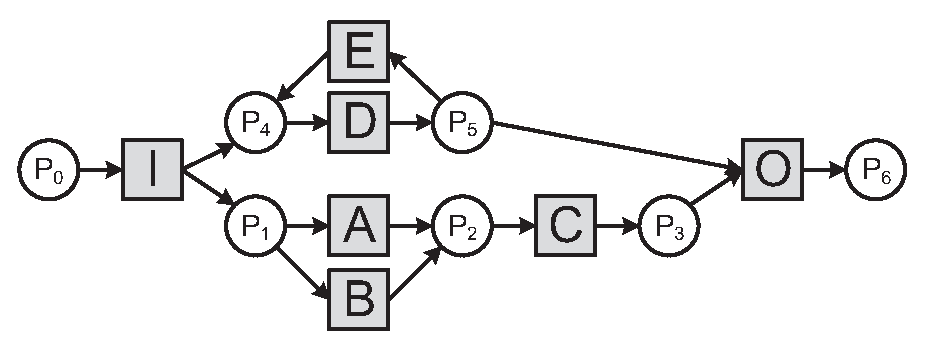
\includegraphics[width=1\textwidth]{fig_example_petri.eps}
		\label{fig:examplePetri}
	\end{minipage}
}
\subfigure[] {
	\begin{minipage}[b]{0.7\textwidth}
		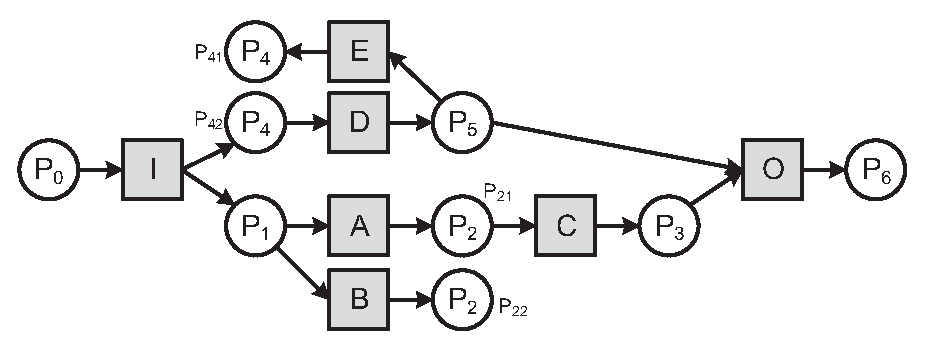
\includegraphics[width=1\textwidth]{fig_example_cpu.eps}
		\label{fig:exampleCpu}
	\end{minipage}
}
\caption{A sound WF-net example and its complete prefix unfolding}
\label{fig:examplePetriAndCpu}
\end{figure}

\begin{example}\label{ex:petriAndCpu}
Fig. \ref{fig:examplePetriAndCpu} shows a sound WF-net and its complete prefix unfolding. In the unfolding in Fig. \ref{fig:exampleCpu}, transitions labelled as $B$ and $E$ are cutoff transitions.
\end{example}

Our extended relations are inspired by the work in \cite{van2006decserflow}, which utilizes the relations between activities to model a process. We use part of the relations in this paper.
\begin{definition}[Relation Formulas]\label{def:relationFormulas}
Let $A$ and $B$ be two activities of a process, $A$ and $B$ are in the following relation formulas:\footnote{Note that the relation formulas are not complete here, since we only need part of them. For more details, please refer to the work of Alast \cite{van2006decserflow}.}
	\begin{itemize}
		\item[-] Responded Existence: if activity $A$ is executed, activity $B$ also has to be executed either before or after the activity $A$.
		\item[-] Co-existence: if one of activities $A$ or $B$ is executed, the other one has to executed also.
		\item[-] Response: every time activity $A$ executes, activity $B$ has to be executed after it.
		\item[-] Precedence: if activity $B$ was executed, it could not have been executed until the activity $A$ was executed.
		\item[-] Alternate Response: after the execution of an activity $A$ activity $B$ has to be executed and between the execution of each two $A$ at least one activity $B$ has to be executed.
		\item[-] Alternate Precedence: every instance of activity $B$ has to be preceded by an instance of activity $A$ and the next instance of activity $B$ cannot be executed before the next instance of activity $A$ is executed.
	\end{itemize}
\end{definition}

\begin{example}\label{ex:relationFormulas}
Let $A,B,C$ be activities of a process. The execution sequence $[B,A,A,A,C,B]$ satisfies the formula \textit{response}; The execution sequence $[A,C,B,B,A]$ satisfies the formula \textit{precedence}; The execution sequence $[B,A,C,B,A,B]$ satisfies the formula \textit{alternate response}; The execution sequence $[A,C,B,A,B,A]$ satisfies the formula \textit{alternate precedence}.
\end{example}

\section{Extended Refined Ordering Relations with Uncertainty}\label{sec:relations}
In this section, we introduce the concept of extended refined ordering relations with uncertainty and its calculation from a WF-net. Let $\Sigma=(P,T,F,M_{0})$ be a sound WF-net, and $A,B\in T$ be transitions of the WF-net. A path means a directed path from the source place to the sink place in the WF-net. Let $S$ be the set containing all the paths of the WF-net, and $S_{A}$ be the set of the paths containing transition $A$, i.e, $S_{A}=\{\sigma\in S|A\in\sigma\}$. Our extended relations are defined using the notion of $S_{A}$.

\subsection{Extended Refined Causal and Inverse Causal Relations with Uncertainty}\label{subsec:causalAndInverseCausal}
Based on whether one task is always executed in the same firing sequence before or after the other task, we extend the causal relations and define new inverse causal relations.

\begin{definition}[Always Causal]\label{def:alwaysCausal}
$A$ and $B$ are in always causal relation (denoted as $A\twoheadrightarrow B$) iff: $\forall\sigma_{A}\in S_{A}$, $A$ and $B$ are in \textit{alternate response} relation, i.e., among all the paths containing transition $A$, after the execution of every $A$ there must be at least one $B$ executed, and before that $B$ there cannot be another transition $A$.
\end{definition}

\begin{definition}[Never Causal]\label{def:neverCausal}
$A$ and $B$ are in never causal relation (denoted as $A\nrightarrow B$) iff: $\forall\sigma_{A}\in S_{A}$, there is no $B$ or $A$ and $B$ are not in \textit{response} relation, i.e., among all the paths containing transition $A$, after the execution of every $A$, there mustn't be an instance of $B$ executed.
\end{definition}

\begin{definition}[Sometimes Causal]\label{def:sometimesCausal}
$A$ and $B$ are in sometimes causal relation (denoted as $A\rightharpoonup B$) iff: $\forall\sigma_{A}\in S_{A}$, $A$ and $B$ are neither in always causal relation nor never causal relation.
\end{definition}

\begin{example}\label{ex:causalRelation}
In the model of Fig. \ref{fig:examplePetri}, $A$ and $C$ are in \textit{always causal} relation ($A\twoheadrightarrow C$) since they are in \textit{alternate response} relation among all the paths containing $A$. $D$ and $O$ are in \textit{sometimes causal} relation ($D\rightharpoonup O$) since there may be another $D$ between the execution of the first $D$ and $O$, indicating that $D$ and $O$ are not in \textit{alternate response} relation. $C$ and $D$ are in \textit{never causal} relation ($C\nrightarrow D$).
\end{example}

\begin{definition}[Always Inverse Causal]\label{def:alwaysInverseCausal}
$A$ and $B$ are in always inverse causal relation (denoted as $B\twoheadrightarrow^{-1}A$) iff: $\forall\sigma_{B}\in S_{B}$, $A$ and $B$ are in \textit{alternate precedence} relation, i.e., among all the paths containing transition $B$, every instance of $B$ has to be preceded by an instance of $A$ and the next instance of transition $B$ cannot be executed before the next instance of transition $A$ is executed.
\end{definition}

\begin{definition}[Never Inverse Causal]\label{def:neverInverseCausal}
$A$ and $B$ are in never inverse causal relation (denoted as $B\nrightarrow^{-1}A$) iff: $\forall\sigma_{B}\in S_{B}$, there is no $A$ or $A$ and $B$ are not in \textit{precedence} relation, i.e., among all the paths containing transition $B$, before the execution of every $B$, there mustn't be an instance of $A$ executed.
\end{definition}

\begin{definition}[Sometimes Inverse Causal]\label{def:sometimesInverseCausal}
$A$ and $B$ are in sometimes inverse causal relation (denoted as $B\rightharpoonup^{-1}A$) iff: $\forall\sigma_{B}\in S_{B}$, $A$ and $B$ are neither in always inverse causal relation nor never inverse causal relation.
\end{definition}

\begin{example}
In the model of Fig. \ref{fig:examplePetri}, $D$ and $O$ are in \textit{always inverse causal} relation ($O\twoheadrightarrow^{-1}D$) since they are in \textit{alternate precedence} relation among all the paths containing $O$. $A$ and $C$ are in \textit{sometimes inverse causal} relation ($C\rightharpoonup^{-1}A$) since there may be no instance of transition $A$ in some paths containing $C$, indicating that $A$ and $C$ are not in \textit{precedence} relation. $C$ and $D$ are in \textit{never inverse causal} relation ($D\nrightarrow^{-1}C$).
\end{example}

We have identified several scenarios of causal and inverse causal relation and turn them into abstract formulas, as shown in Fig. \ref{fig:causalCases}.

\begin{figure}[!htb]
\centering
\subfigure[] {
	\begin{minipage}[b]{0.45\textwidth}
		\centering
		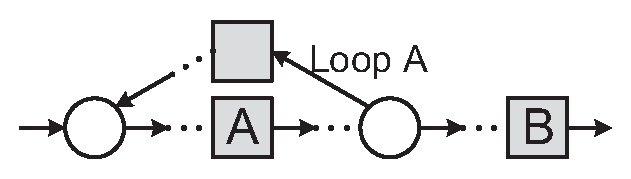
\includegraphics[width=0.8\textwidth]{fig_causal_case_a_1.eps}\\
		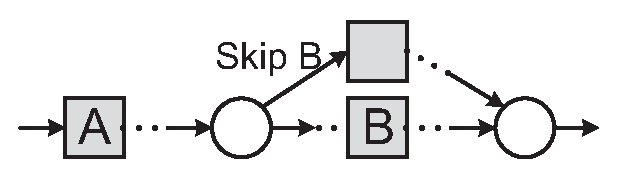
\includegraphics[width=0.8\textwidth]{fig_causal_case_a_2.eps}
	\end{minipage}
	\label{fig:causalCaseA}
}
\subfigure[] {
	\begin{minipage}[b]{0.45\textwidth}
		\centering
		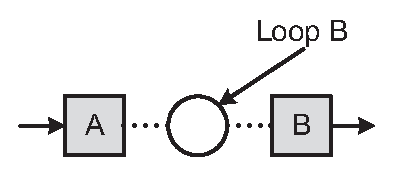
\includegraphics[width=0.8\textwidth]{fig_causal_case_b_1.eps}
		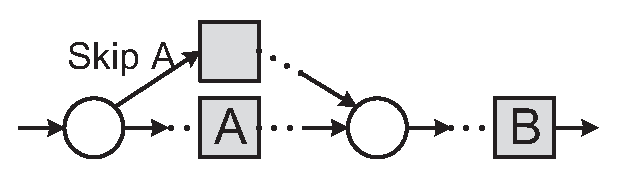
\includegraphics[width=0.8\textwidth]{fig_causal_case_b_2.eps}
	\end{minipage}
	\label{fig:causalCaseB}
}
\subfigure[] {
	\begin{minipage}[b]{0.45\textwidth}
		\centering
		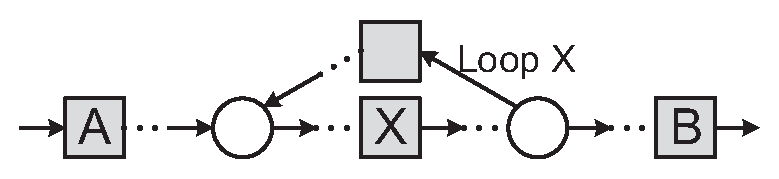
\includegraphics[width=1\textwidth]{fig_causal_case_c.eps}
	\end{minipage}
	\label{fig:causalCaseC}
}
\subfigure[] {
	\begin{minipage}[b]{0.45\textwidth}
		\centering
		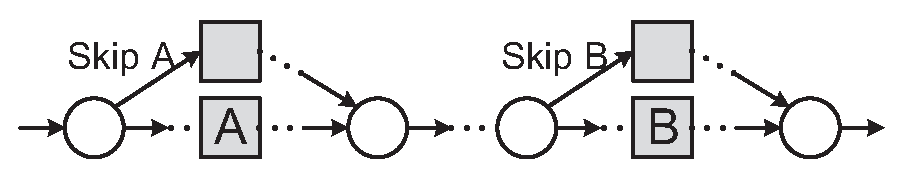
\includegraphics[width=1\textwidth]{fig_causal_case_d.eps}
	\end{minipage}
	\label{fig:causalCaseD}
}
\caption{Abstract formulas of causal and inverse causal relations. \subref{fig:causalCaseA} $A\rightharpoonup B, B\twoheadrightarrow^{-1}A$; \subref{fig:causalCaseB} $A\twoheadrightarrow B, B\rightharpoonup^{-1}A$; \subref{fig:causalCaseC} $A\twoheadrightarrow B, B\twoheadrightarrow^{-1}A$; \subref{fig:causalCaseD} $A\rightharpoonup B, B\rightharpoonup^{-1}A$.}
\label{fig:causalCases}
\end{figure}

\subsection{Extended Refined Concurrent Relations with Uncertainty}\label{subsec:concurrent}
Based on whether one task is always executed in the same firing sequence concurrently with the other task, we extend the causal relations and define new inverse causal relations.

\begin{definition}[Always Concurrent]\label{def:alwaysConcurrent}
\end{definition}

\begin{definition}[Never Concurrent]\label{def:neverConcurrent}
\end{definition}

\begin{definition}[Sometimes Concurrent]\label{def:sometimesConcurrent}
\end{definition}

\subsection{Computing Extended Refined Ordering Relations Based on Unfolding}\label{subsec:computationOfRelations}
In Section \ref{subsec:causalAndInverseCausal} and Section \ref{subsec:concurrent}, we give the definitions of extended refined ordering relations with uncertainty. In this section, we focus on the computation of our relations for the unfolding of sound WF-net.

As mentioned before, an intuitive idea to derive our relations is based on reachability graphs. Such technique would face a state explosion problem, especially when the WF-net contains a parallel with large scale of transitions. Theoretically, the reachability graph will derive all the reaching states by combining the executions of transitions within a parallel structure. What's more important is that we actually cannot distinguish the relation of \textit{response} and \textit{alternate response} in a WF-net with loop structure using the reachability technique. So we adopt the unfolding technology in this paper.

The reason why we do not derive the relations based on sound WF-net itself is that WF-net describe the structure of process rather than behaviors, which is the focus of unfolding technique. In the complete prefix unfolding of the WF-net, there would be cutoff transitions and cutoff places (places after those cutoff transitions). We need to find out all the cutoff places pointing to the gate of a loop structure to avoid that we traverse the loop part again and again. By traversing along the path between two specific transitions, we can derive the extended ordering relations between them, which will be specified later.

We may notice the fact that the computations of causal relation and inverse causal relation are similar in the way that we regard inverse causal relation as causal relation in the reversion of the WF-net. In another word, if we reverse the direction of every edge in the WF-net, then the causal relations in the new WF-net are the same as the inverse causal relations in the original WF-net. This indicates that we can use the algorithm of causal relations to derive the inverse causal relations by backtracing nodes along the paths of a WF-net.

There may be more than one corresponding event (a.k.a. shadow event) in the complete prefix unfolding of a transition in the original WF-net. Therefore, when we derive the extended ordering relation between transition $A$ and $B$, we need to check the relations between each shadow event of $A$ and some shadow event of $B$. For example, $A\twoheadrightarrow B$ is said to be true if and only if $\forall a\in\{shadow~events~of~A\}, \exists b\in\{shadow~events~of~B\}, a\twoheadrightarrow b$.

The computation of extended causal relations is listed as Algorithm.

\begin{algorithm}[!htb]
\caption{Computation of Extended Causal Relations}\label{algo:causal}
\begin{algorithmic}[1]
\Require A sound WF-net $\Sigma=(P,T,F,M_{0})$ and its complete prefix unfolding $\beta=(B,E,A,f)$
\Ensure xxx
\end{algorithmic}
\end{algorithm}


% \section{Similarity Measure}\label{sec:similarity}

% \section{Experiments}\label{sec:experiments}

% \section{Conclusion}\label{sec:conclusion}


\bibliographystyle{plain}
\bibliography{ref}
\end{document}